\subchapter{Filesystem optimizations}{See what best filesystem options
are in terms of boot time}

During this lab, we will compare 3 ways of accessing the root filesystem

\begin{itemize}
\item Booting from an {\em ext4} filesystem
\item Booting from a {\em SquashFS} filesystem
\item Booting from an {\em initramfs}
\end{itemize}

\section{Tests with ext4 and SquashFS}

First, recompile your kernel with built-in {\em SquashFS} support (with
default options), and update it on the SD card.

Write the size of the \code{zImage} file in the first row of the
\code{~/boot-time-labs/results/filesystems-size.ods} spreadsheet:

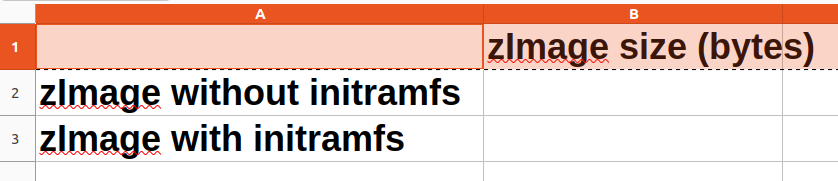
\includegraphics[width=0.6\textwidth]{labs/boot-time-filesystem-optimizations/filesystems-size.png}

Boot your system with \code{grabserial}, copying its output to
\code{~/logs/filesystem-ext4.log}, and start filling the table below:

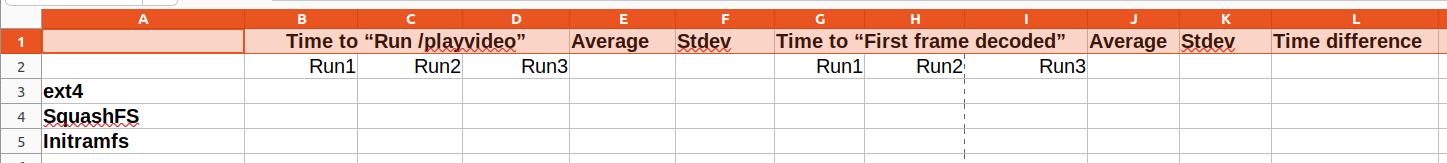
\includegraphics[width=\textwidth]{labs/boot-time-filesystem-optimizations/filesystems-time.png}

For {\em SquashFS}, configure Buildroot to generate a SquashFS image too
(with the default options).

Once this image is generated, you'll just have to update the root
partition from the host machine:

\begin{verbatim}
sudo umount /dev/mmcblk0p2
sudo dd if=rootfs.squashfs of=/dev/mmcblk0p2
\end{verbatim}

Then remove the SD card and boot the board with it as usual, and record
and store measurements.

Note that we also made tests with {\em ext2}, but they were very close
to {\em ext4} ones, at least for very small filesystems like this one.
So we decided to skip this filesystem here, to save time.

\section{Testing further filesystems}

If you have time, you could also test the {\em Btrfs}, {\em F2FS} and
{\em EROFS} filesystems. That's very easy to do, as Buildroot can build
images for such filesystems for you.

\section{Initramfs tests}

Booting from an {\em initramfs} is completely different. The strong
advantage here is that the root filesystem will be extracted from an
archive inside the kernel binary. So instead of several reads from the
MMC, we will just have a single one (though bigger), in addition to the
Device Tree binary.  This can work well with small root filesystems as ours.

Booting the kernel should be faster too, as we won't need the MMC and
filesystem drivers at all. So, let's configure the kernel accordingly.

To switch to an initramfs, there are a few things to do though:
\begin{itemize}
\item In an initramfs, you cannot have the kernel mount the {\em
devtmpfs} filesystem mounted automatically on \code{/dev}. We'll mount
it from our \code{playvideo} script.
So:
   \begin{itemize}
   \item Modify the BusyBox configuration to add support for the
   \code{mount} command (found in \code{Linux System Utilities}), without
    any additional option.
   \item Add the following line to the beginning of the \code{/playvideo} file:\\
   \code{mount -t devtmpfs nodev /dev}
   \item Run \code{make} to update your root filesystem.
   \item Then extract again it in a new \code{rootfs} directory:
\begin{verbatim}
mkdir ../rootfs
cd ../rootfs
tar xvf ../buildroot/output/images/rootfs.tar
\end{verbatim}
   \end{itemize}
\item Go to the U-Boot command line on your board, and modify the
kernel parameters:\\
   \code{setenv bootargs console=ttyS0,115200n8 rdinit=/playvideo}\\
   \code{root=} and \code{rootwait} are ignored when there is an
   Initramfs and \code{init} is replaced by \code{rdinit=}.
   Don't forget to run \code{saveenv}.
\end{itemize}

Go to \code{~/boot-time-labs/kernel/linux} and run the Linux
configuration interface:

\begin{itemize}
  \item In \code{General setup}
  \begin{itemize}
     \item Fill \code{Initramfs source file(s)} with
\code{../../rootfs/rootfs} (or the correct path to the directory
containing your root filesystem)
     \item Make sure you set \kconfigval{CONFIG_INITRAMFS_COMPRESSION_NONE}{y}
	   to avoid wasting space compressing the initramfs twice.
  \end{itemize}
  \item Disable \code{Enable the block layer}
  \item In \code{Device Drivers}, disable \code{MMC/SD/SDIO card support}
  \item We won't have to disable block filesystems as they are no longer
compiled when block support is disabled.
\end{itemize}

Rebuild your kernel binary:
\begin{verbatim}
make -j8 zImage
\end{verbatim}

Copy the new kernel image to your SD card and then boot the board. You
will see that there is a new issue though: the messages from \code{echo}
and \code{ffmpeg} don't go through. That's probably because
\code{/dev/console} doesn't exit yet when the script is started.

So, let's fix it in our script. We are redirecting the important
messages to \code{/dev/console}:

{\scriptsize
\begin{verbatim}
#!/bin/sh
mount -t devtmpfs nodev /dev
if ! [ -e /dev/video0 ]
then
   echo "Waiting for /dev/video0 to be ready..." > /dev/console
   while ! [ -e /dev/video0 ]
   do
       usleep 1000
   done
fi
echo "Starting ffmpeg" > /dev/console
ffmpeg -t 10 -f video4linux2 -video_size 544x288 -input_format mjpeg -i /dev/video0 -pix_fmt rgb565le -f fbdev /dev/fb0 2> /dev/console
\end{verbatim}
}

Now, you should be able to extract the measures and write them down in
the table above. If your tests run the same way ours did, the
initramfs approach should win by a few tens of milliseconds.

Also measure the size of your \code{zImage} file and write it in the
\code{filesystems-size.ods} spreadsheet, to compare with your initial kernel.

Let's choose this solution with an initramfs. There are still many things we can
accelerate during the execution of the bootloader and execution.
